\section{Two dimensions: the smoothed Riesz identity}\label{bsy:sec:2d}

The one dimensional rule stalls between $N^{-1/2}$ and $N^{-2/3}$ because the Cauchy kernel has a heavy tail and $\log|\zeta|$ never stops oscillating. Both come from the boundary formulation: Theorem~\ref{bsy:thm:bsy} tests $\log|h_\theta|$ against the Green function of a half plane, whose normal derivative on the line is $2\pi$ times the Cauchy density. Testing against a smooth bump of compact support instead gives an identity with no tail at all, at the price of one more dimension.

\begin{theorem}[smoothed Riesz identity]\label{bsy:thm:riesz2d}
Let $f$ be meromorphic on a neighbourhood of a compact set $K\subset\mathbb{C}$, not identically zero on any component of the neighbourhood, and let $\varphi\in C_c^\infty$ with support in $K$. Then
\[
I(\varphi):=\iint\log|f(\sigma+it)|\,\Delta\varphi(\sigma,t)\,d\sigma\,dt=2\pi\Bigl(\sum_{f(\rho)=0}\varphi(\rho)-\sum_{f(p)=\infty}\varphi(p)\Bigr),
\]
with zeros and poles counted with multiplicity. Equivalently, for $f=\xi$,
$-\iint\bigl(\pi\,m_\sigma(t)\,\partial_\sigma\varphi+\partial_t\log|\xi|\,\partial_t\varphi\bigr)\,d\sigma\,dt=2\pi\sum\varphi(\rho)$, so the Thorin density $m_\sigma$ is the $\sigma$ component of the field whose divergence counts the zeros.
\end{theorem}

\begin{proof}
In the sense of distributions $\Delta\log|f|=2\pi\bigl(\sum\delta_\rho-\sum\delta_p\bigr)$, because $\log|f|=\log|g|+\sum\log|s-\rho|-\sum\log|s-p|$ with $g$ analytic and zero free near $K$, $\log|g|$ harmonic, $\Delta\log|s-\rho|=2\pi\delta_\rho$ and $\Delta\log|s-p|^{-1}=-2\pi\delta_p$ at a pole. Pair with $\varphi$ and integrate by parts twice. The second form is one integration by parts, with $\partial_\sigma\log|\xi|=\pi m_\sigma$ (equation~\eqref{lo:eq:Utheta} and Theorem~\ref{lo:thm:density}); $\nabla\log|\xi|$ is locally integrable since its singularities are of order $1/|s-\rho|$.
\end{proof}

Theorem~\ref{bsy:thm:bsy} corresponds formally to taking for $\varphi$ the Green function of $\{\Re s>\theta\}$ with pole at $1+it_0$, which is singular at the pole and not compactly supported; integrating out $\sigma$ leaves the Cauchy average on the line. With a bump instead, both obstacles of the one dimensional rule disappear. If $f$ has no zeros in the support, $g=\log|f|\,\Delta\varphi$ is in $C_c^\infty$ and $I(\varphi)=0$ exactly; a zero $\rho$ in the support moves $I$ by $2\pi\varphi(\rho)$, of order one unless $\rho$ is near the edge. With a partition of unity $\sum_k\varphi_k=1$ on a region, $\sum_kI(\varphi_k)=2\pi$ times the number of zeros in the region, plus $2\pi\sum_k\varphi_k(\rho)$ for each zero $\rho$ where $0<\sum_k\varphi_k<1$, so overlapping bumps leave no blind spots.

\subsection{Weighted Monte Carlo in the plane}

Map the box to $[-1,1]^2$ and take $\varphi(x,y)=b(x)b(y)$ with $b(x)=e^{-1/(1-x^2)}$ on $|x|<1$. The rules we compare all use $N$ nodes:
\begin{enumerate}\setlength{\itemsep}{1pt}
\item plain Monte Carlo, the sample mean at uniform nodes;
\item Voronoi weights: each uniform node is weighted by the area of its Voronoi cell, the two dimensional form of weighting by spacings;
\item Delaunay weights: piecewise linear interpolation on the Delaunay triangulation of the nodes and the four corners, the two dimensional trapezoid rule; at uniform nodes and at jittered nodes, one uniform point in each cell of a $\sqrt N\times\sqrt N$ grid;
\item the randomly shifted product trapezoid rule on a $\sqrt N\times\sqrt N$ grid;
\item deflation: replace $\log|f|$ by $\log|f(s)/(s-\hat\rho)|$ for an estimate $\hat\rho$ of a zero, and add back $2\pi\varphi(\hat\rho)$, which is exact by Theorem~\ref{bsy:thm:riesz2d} for meromorphic $f$.
\end{enumerate}
All of these are unbiased or asymptotically unbiased, and the spread over replications estimates their random error, not their bias.

\begin{proposition}[rates]\label{bsy:prop:rates2d}
After an affine change of variables the box is the torus $[0,1)^2$; the shifted product trapezoid rule with $N=m^2$ nodes is $Q(\delta)=m^{-2}\sum_{j\in\{0,\dots,m-1\}^2}g(j/m+\delta)$, with $\delta$ uniform on $[0,1/m)^2$.
(i) If $g$ has a smooth periodic extension (for example the integrand $\log|f|\,\Delta\varphi$ with the flat bump of the text and no zero in the box), then $Q(\delta)-\int g=O(N^{-k})$ for every $k$, uniformly in $\delta$, and $\E_\delta Q=\int g$.
(ii) If $g=\psi\log|s-\rho|$ with $\psi\in C_c^\infty((0,1)^2)$ and $\rho\in(0,1)^2$, then $\E_\delta Q=\int g$ and $\bigl(\E_\delta|Q-\int g|^2\bigr)^{1/2}=O(N^{-1})$. For a fixed shift whose nodes all lie at distance at least $c/m$ from $\rho$, $|Q-\int g|=O_c(N^{-1}\log N)$. If $\psi(\rho)\ne0$, no bound uniform in the shift holds.
(iii) On the box, for $g$ as in Theorem~\ref{bsy:thm:wmc} (for example the integrand of the text when $f$ has no zero in the closed box), Voronoi weights and Delaunay weights at independent uniform nodes have root mean square error $O(N^{-3/2})$, against $N^{-1/2}$ for the sample mean (Theorem~\ref{bsy:thm:wmc}); at jittered nodes the same rate is computed, not proved.
\end{proposition}

\begin{proof}
For $g$ square integrable on the torus, Poisson summation gives, in $L^2(d\delta)$, $Q(\delta)-\int g=\sum_{\ell\ne0}\hat g(m\ell)\,e^{2\pi im\langle\ell,\delta\rangle}$ with $\hat g(k)=\int g(x)e^{-2\pi i\langle k,x\rangle}dx$. These exponentials are orthonormal for $\delta$ uniform on $[0,1/m)^2$, so $\E_\delta Q=\int g$ and $\E_\delta|Q-\int g|^2=\sum_{\ell\ne0}|\hat g(m\ell)|^2$. (i) $\hat g$ decays faster than every power, and the series converges absolutely, uniformly in $\delta$. (ii) In the sense of distributions $\Delta g=2\pi\psi(\rho)\delta_\rho+q$ with $q=2\nabla\psi\cdot\nabla\log|s-\rho|+\Delta\psi\,\log|s-\rho|\in L^1$, so $4\pi^2|k|^2|\hat g(k)|\le2\pi|\psi(\rho)|+\|q\|_1$ and $\E_\delta|Q-\int g|^2\le Cm^{-4}\sum_{\ell\ne0}|\ell|^{-4}=O(N^{-2})$. For the separated bound put $h=1/m$: on a cell at distance $r\ge2h$ from $\rho$ the trapezoid error is $O(h^4r^{-2})$, and the $O(r\,dr/h^2)$ cells at distance about $r$ give $O(h^2\log(1/h))$ in total; the $O(1)$ cells within $2h$ of $\rho$ contribute $O(h^2\log(1/h))$ to $\int g$ and, by the separation, $O(h^2\log(1/(ch)))$ to $Q$. If $\psi(\rho)\ne0$, a node at distance $\eta$ from $\rho$ contributes $m^{-2}\psi(\rho)\log\eta+O(m^{-2})$, which is unbounded as $\eta\to0$, so no bound uniform in $\delta$ holds. (iii) is Theorem~\ref{bsy:thm:wmc} with $d=2$.
\end{proof}

\subsection{A proof of the $N^{-3/2}$ rate}\label{bsy:sec:wmc}

The rate of Proposition~\ref{bsy:prop:rates2d}(iii) holds at independent uniform nodes in every dimension, for the Voronoi rule and for the Delaunay rule with the corners of the box added. Write $x_{\mathrm{nn}}(x)$ for the node nearest to $x$, $d(x)=|x-x_{\mathrm{nn}}(x)|$ and $v(x)=x_{\mathrm{nn}}(x)-x$. Then $\frac12d(x)^2=\frac12|x|^2-\max_i\bigl(x\cdot X_i-\frac12|X_i|^2\bigr)$ is Lipschitz with gradient $-v(x)$ almost everywhere, so the displacement to the nearest node is a gradient field, and the first order error of the Voronoi rule integrates by parts into a second order quantity.

\begin{theorem}[weighted Monte Carlo for integrands flat at the boundary]\label{bsy:thm:wmc}
Let $Q=[-1,1]^d$, let $X_1,\dots,X_N$ be independent and uniform on $Q$, and let $g\in C^3(Q)$ satisfy (a) $g=0$ within distance $\delta>0$ of $\partial Q$, or (b) $g\in C^\infty(Q)$ with every derivative vanishing on $\partial Q$. Let $V_N=\sum_i|V_i\cap Q|\,g(X_i)$ be the Voronoi rule, with the cells clipped to $Q$, and $D_N=\int_QI_Ng$ the Delaunay rule, where $I_Ng$ interpolates $g$ linearly on the Delaunay triangulation of the nodes and the $2^d$ corners of $Q$. Then
\begin{align*}
V_N-\int_Qg&=\frac12\int_Qd(x)^2\,\Delta g(x)\,dx+\frac12\int_Qv^{\mathsf T}D^2g(x)\,v\,dx+\int_Qr(x)\,dx,\\
|r(x)|&\le\tfrac16\|D^3g\|_\infty|v|^3,
\end{align*}
and for $A_N=V_N$ and for $A_N=D_N$
\[
\Bigl|\E A_N-\int_Qg\Bigr|=\begin{cases}O(Ne^{-cN\delta^d})&\text{in case (a)},\\ O(N^{-k})\ \text{for every }k&\text{in case (b)},\end{cases}\qquad\mathrm{Var}\,A_N=O(N^{-1-4/d}).
\]
So the root mean square error is $O(N^{-1/2-2/d})$ in every dimension: $N^{-5/2}$ on the line and $N^{-3/2}$ in the plane. The constants depend on $g$, $d$ and, in case (a), $\delta$. Case (b) includes $g=\log|f|\,\Delta\varphi$ for the bump $\varphi$ of Section~\ref{bsy:sec:2d}, mapped to $Q$, when $f$ is analytic and zero free on a neighbourhood of the closed box.
\end{theorem}

\begin{proof}
Identity. The Voronoi rule is $\int_Qg(x_{\mathrm{nn}}(x))\,dx$, so its error is $\int_Q[g(x+v)-g(x)]\,dx$; expand to third order. The first order term is $\int_Q\nabla g\cdot v=-\int_Q\nabla g\cdot\nabla(\frac12d^2)=\frac12\int_Qd^2\Delta g$, with no boundary term because $\nabla g=0$ on $\partial Q$ in both cases.

Bias of the Voronoi rule. By exchangeability $\E V_N=\int_Qg(y)\,w_N(y)\,dy$ with
\[
w_N(y)=\frac N{|Q|}\int_Q\Bigl(1-\frac{|B(x,|x-y|)\cap Q|}{|Q|}\Bigr)^{N-1}dx,
\]
which is $N/|Q|$ times the expected volume of the cell of a node placed at $y$. Let $r=\frac12\mathrm{dist}(y,\partial Q)$ and $\kappa_d=|B(0,1)|$. For $|x-y|\le r$ the ball $B(x,|x-y|)$ lies in $Q$ and the integrand is $(1-\kappa_d|x-y|^d/|Q|)^{N-1}$. For $x\in Q$ and $\rho\le2$, $|B(x,\rho)\cap Q|\ge4^{-d}\kappa_d\rho^d$ (for $\rho\le1$ the ball contains its part in the orthant at $x$ that points to the centre of $Q$, which lies in $Q$, and for $1<\rho\le2$ use the radius $1$), so for $|x-y|>r$ the integrand is at most $e^{-c_1Nr^d}$. Since $\frac N{|Q|}\int_{\R^d}(1-\kappa_d|u|^d/|Q|)_+^{N-1}du=N\int_0^1(1-t)^{N-1}dt=1$ and the two integrands agree for $|x-y|\le r$, $|w_N(y)-1|\le CNe^{-c_1Nr^d}$. Hence $|\E V_N-\int_Qg|\le CN\int_Q|g(y)|\,e^{-c_1N(\mathrm{dist}(y,\partial Q)/2)^d}\,dy$. In case (a) this is $O(Ne^{-c_1N(\delta/2)^d})$. In case (b) Taylor's formula at the nearest boundary point gives $|g(y)|\le C_m\,\mathrm{dist}(y,\partial Q)^m$ for every $m$, and the bound is $O(N^{1-(m+1)/d})$ for every $m$.

Variance of the Voronoi rule. Let $R$ be the largest distance from a node to the points of its clipped cell. If $R>\rho$ for a node $y$, the convex cell contains a point $x$ with $|x-y|=\rho$, and $B(x,\rho)$ holds no other node; one of a fixed set of $C_d$ points $x'$ on the sphere $|x'-y|=\rho$ has $|x-x'|\le\frac\rho4$, and then $B(x,\frac\rho2)\subset B(x',\frac34\rho)\subset B(x,\rho)$, so $B(x',\frac34\rho)$ holds no other node and, as $x\in Q$, meets $Q$ in volume at least $4^{-d}\kappa_d(\rho/2)^d$. So $P(R>\rho\mid y)\le C_de^{-cN\rho^d}$ for $\rho\le4$, uniformly in $y$, and $\E R^p=O(N^{-p/d})$ for every $p$. The node nearest to $y$ is at distance at most $2R$, because the midpoint lies in the cell of $y$; so removing $y$ moves the nearest node of each point of its cell to distance at most $3R$. Write $V_N-\int_Qg=\int_Q\frac12d^2\Delta g\,dx+\int_Q\mathcal R(x,v(x))\,dx$ with $\mathcal R(x,v)=g(x+v)-g(x)-\nabla g(x)\cdot v$, $|\mathcal R|\le\frac12\|D^2g\|_\infty|v|^2$. Replacing $X_1$ by an independent copy $X_1'$ changes the integrands only on the old cell of $X_1$ and the new cell of $X_1'$, where $d$ and $|v|$ are at most $3\max(R,R')$ before and after, $R$ and $R'$ being the two cell radii. So $|V_N-V_N'|\le C(R^{d+2}+R'^{d+2})$, $\E(V_N-V_N')^2=O(N^{-2-4/d})$, and the Efron and Stein inequality gives $\mathrm{Var}\,V_N\le\frac N2\E(V_N-V_N')^2=O(N^{-1-4/d})$.

The Delaunay rule. Linear interpolation has no first order error, since $\sum_j\lambda_j(x)(y_j-x)=0$ for the barycentric coordinates of $x$ in its simplex $S$, and $|I_Ng-g|\le\frac12\|D^2g\|_\infty\,\mathrm{diam}(S)^2$ on $S$, whatever the shape of $S$. In case (a) identify opposite faces of $Q$ to make a flat torus, on which $g$ extends smoothly. There the Delaunay weights $w_i=\int\lambda_i$ are nonnegative, sum to $|Q|$ and move with translations of the configuration, so $\E(w_i\mid X_i=x)=|Q|/N$ and the torus rule is exactly unbiased. Fix $\eta$ small compared with $\delta$. Outside an event of probability $O(e^{-cN\eta^d})$ every ball of radius $\eta$ in a fixed finite net inside $Q$ contains a node. On that event the empty circumball of a simplex that meets the support of $g$ has radius $O(\eta)$, because it contains a ball inside $Q$ of radius comparable to the smaller of its radius and $\delta$; so the simplices that carry $g$, and the weights of the nodes in the support, are the same for the box with its corners and for the torus. Both rules are bounded by $|Q|\,\|g\|_\infty$, so the box rule has bias $O(e^{-cN\delta^d})$. Inserting a node changes the triangulation only in the union of the simplices whose circumballs contain it; on the same event the part of it that carries $g$ lies within a radius $R$ of the node with $P(R>\rho)\le Ce^{-cN\rho^d}$, by the net argument above, and by the value bound the rule changes by $O(R^{d+2})$; the Efron and Stein inequality gives $\mathrm{Var}\,D_N=O(N^{-1-4/d})$ as before. In case (b) write $g=g\chi+g(1-\chi)$ with a cutoff $\chi$ equal to $1$ at distance at least $2\delta_N$ from $\partial Q$ and to $0$ within $\delta_N$, $\delta_N=N^{-1/(2d)}$, whose derivatives of order $j$ are $O(\delta_N^{-j})$. The second part changes both the rule and the integral by at most $|Q|\sup|g(1-\chi)|=O(N^{-k})$ for every $k$, since the weights are nonnegative and sum to $|Q|$. The first part satisfies (a) with $\delta=\delta_N$, so its bias is $O(e^{-cN^{1/2}})$, and its second derivatives are bounded uniformly in $N$, because the derivatives of $g$ within $2\delta_N$ of $\partial Q$ are $O(\delta_N^m)$ for every $m$; so its variance is $O(N^{-1-4/d})$.
\end{proof}

Lemma~\ref{bsy:lem:trap} gives the rate of Yakowitz, Krimmel and Szidarovszky its exact form: their mean square $N^{-4}$ is the squared bias $\frac{(b-a)^4(g'(b)-g'(a))^2}{4N^4}$ to leading order, and when $g'(a)=g'(b)$ the mean square error is $O(N^{-5})$ (for $g\in C^4$ by the lemma, and for $g$ as in Theorem~\ref{bsy:thm:wmc} with $d=1$ by that theorem).

\begin{remark}\label{bsy:rem:flat}
If $g$ is smooth on $Q$ but does not vanish near $\partial Q$, the integration by parts leaves the boundary term $-\frac12\oint_{\partial Q}d^2\,\partial_ng$, and $\int_Q\Delta g=\oint_{\partial Q}\partial_ng$ need not vanish, so the bias of these rules is in general of order $N^{-2/d}$ (affine $g$ is an exception); the exponential rows of Table~\ref{bsy:tab:wmc} show it (computed).
\end{remark}

\begin{table}[h]
\centering\footnotesize\setlength{\tabcolsep}{3pt}
\begin{tabular}{lcccc}
\toprule
integrand and rule & $N=1000$ & largest $N$ & slope & bound\\
\midrule
bump, $d=1$, Voronoi & $1.2\times10^{-6}$ & $3.5\times10^{-14}$ (1{,}024{,}000) & $-2.51$ & $-\frac52$\\
$e^x$, $d=1$, trapezoid & $4.8\times10^{-6}$ & $4.5\times10^{-12}$ (1{,}024{,}000) & $-2.00$ & $-2$\\
bump, $d=2$, Voronoi & $1.4\times10^{-4}$ & $5.1\times10^{-9}$ (1{,}024{,}000) & $-1.46$ & $-\frac32$\\
bump, $d=2$, Delaunay & $1.1\times10^{-4}$ & $4.2\times10^{-9}$ (1{,}024{,}000) & $-1.42$ & $-\frac32$\\
$e^{x+y/2}$, $d=2$, Delaunay & $1.0\times10^{-2}$ & $1.2\times10^{-5}$ (1{,}024{,}000) & $-0.98$ & $-1$\\
\bottomrule
\end{tabular}
\caption{Root mean square error of the weighted rules at independent uniform nodes on $Q=[-1,1]^d$, $200$ replications in one dimension and $30$ in two (about $5$ percent noise in each root mean square error in one dimension and about $13$ percent in two), the largest $N$ in brackets, slopes fitted for $N\ge4000$ (computed, floating point). The bump $\prod_ib(x_i/0.9)$ vanishes near $\partial Q$ (case (a) of Theorem~\ref{bsy:thm:wmc}); the exponentials do not, and their error is the bias of Remark~\ref{bsy:rem:flat}. The slopes are consistent with the last column, the exponent of Theorem~\ref{bsy:thm:wmc}, of Lemma~\ref{bsy:lem:trap} for the trapezoid row and of the Remark for the last row.}\label{bsy:tab:wmc}
\end{table}

\subsection{Results}

The box is $0.6\le\sigma\le1.4$, $83.7\le t\le87.7$, centred on the Davenport and Heilbronn zero at height $85.70$ (Figure~\ref{bsy:fig:maps}). For $\zeta$ there are no zeros in the box, so $I(\varphi)=0$. For Davenport and Heilbronn the box contains $\rho=0.808517182457+85.699348485378\,i$, so $I(\varphi)=2\pi\varphi(\rho)=0.63165631$. Both functions are evaluated by a vectorised Euler and Maclaurin formula, accurate to about $10^{-12}$. Table~\ref{bsy:tab:2d} and Figure~\ref{bsy:fig:rates2d} give root mean square errors.

\begin{figure}[h]
\centering
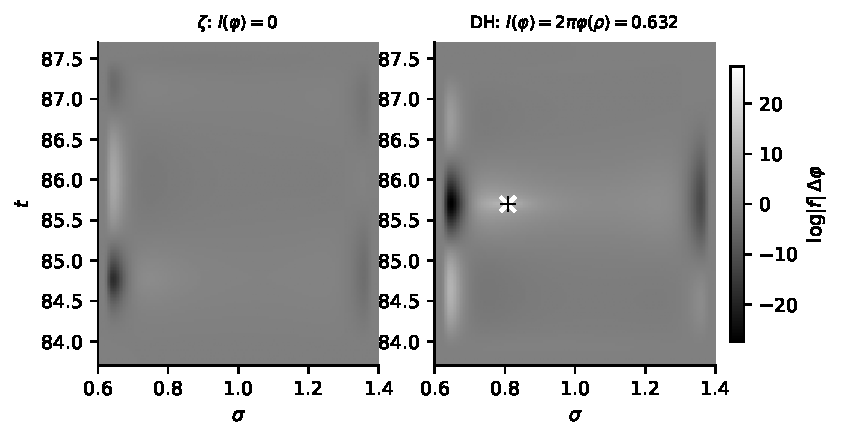
\includegraphics[width=\textwidth]{fig/bsy_riesz2d_maps.pdf}
\caption{The integrand $\log|f|\,\Delta\varphi$ on the box ($121\times121$ points, one grey scale for both functions). The cross marks the Davenport and Heilbronn zero. The large values are at the left and right edges of the box, where $\Delta\varphi$ is largest and $\log|f|$ is large; the picture does not show the zero, which is why the two look alike. Their integrals are $0$ and $0.632$.}\label{bsy:fig:maps}
\end{figure}

\begin{table}[h]
\centering\scriptsize\setlength{\tabcolsep}{2pt}
\begin{tabular}{llcccccc}
\toprule
 & $N$ & plain & Voronoi & Delaunay & jittered & grid & deflated\\
\midrule
$\zeta$ & 1024 & $1.2\times10^{-1}$ & $4.3\times10^{-2}$ & $4.5\times10^{-2}$ & $2.0\times10^{-2}$ & $3.0\times10^{-3}$ & \\
$\zeta$ & 16384 & $3.9\times10^{-2}$ & $1.7\times10^{-3}$ & $1.5\times10^{-3}$ & $4.4\times10^{-4}$ & $1.9\times10^{-6}$ & \\
$\zeta$ & 262144 & $9.0\times10^{-3}$ & $3.2\times10^{-5}$ & $2.4\times10^{-5}$ & $5.6\times10^{-6}$ & $2.2\times10^{-14}$ & \\
\midrule
DH & 1024 & $2.3\times10^{-1}$ & $5.8\times10^{-2}$ & $5.3\times10^{-2}$ & $3.3\times10^{-2}$ & $1.5\times10^{-2}$ & $2.7\times10^{-2}$\\
DH & 16384 & $6.7\times10^{-2}$ & $3.0\times10^{-3}$ & $2.5\times10^{-3}$ & $1.0\times10^{-3}$ & $6.9\times10^{-4}$ & $1.5\times10^{-5}$\\
DH & 262144 & $1.2\times10^{-2}$ & $9.5\times10^{-5}$ & $7.4\times10^{-5}$ & $6.1\times10^{-5}$ & $4.8\times10^{-5}$ & $3.5\times10^{-6}$\\
\bottomrule
\end{tabular}
\caption{Root mean square error of $I(\varphi)$ (computed, floating point, $20$ replicates; the relative standard error of an entry is $16\%$). Jittered is Delaunay on jittered nodes; deflated grid uses an estimate of the zero that is off by $1.4\times10^{-4}$, along $(1+i)/\sqrt2$.}\label{bsy:tab:2d}
\end{table}

\begin{figure}[h]
\centering
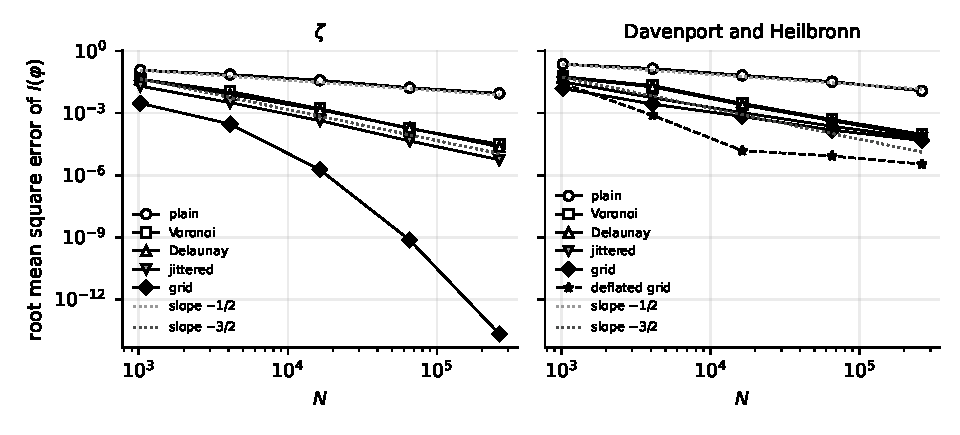
\includegraphics[width=\textwidth]{fig/bsy_riesz2d_rates.pdf}
\caption{Root mean square error of $I(\varphi)$ against $N$ in two dimensions, $20$ replicates, for $\zeta$ (left) and Davenport and Heilbronn (right), with the plain, Voronoi, Delaunay, jittered, grid and (Davenport and Heilbronn) deflated grid rules, the deflating zero being off by $1.4\times10^{-4}$. The dotted lines have slopes $-\frac12$ and $-\frac32$.}\label{bsy:fig:rates2d}
\end{figure}

The fitted slopes for $N\ge4096$ are consistent with Proposition~\ref{bsy:prop:rates2d}. For $\zeta$, with no zero in the box, they are $-0.51$ for plain Monte Carlo, $-1.43$ for Voronoi weights, $-1.40$ for Delaunay weights and $-1.54$ for Delaunay at jittered nodes (the observed slopes lie between $-1.4$ and $-1.55$, so $N^{-3/2}$ is an upper estimate). The shifted grid falls faster than any power, to $2.2\times10^{-14}$ at $N=262{,}144$, the accuracy of the function values. So the spacings rule gains a factor $N$ over plain sampling (proved at independent uniform nodes, Theorem~\ref{bsy:thm:wmc}; computed at jittered nodes) and the grid is limited only by arithmetic. This answers, in two dimensions, the question raised at the start of Section~\ref{bsy:sec:halfdisk}: the change that makes the integrand smooth is not a change of variable on the line but a move off it.

With a zero in the box the logarithmic singularity takes over at large $N$. All the weighted rules slow to slopes between $-1.0$ and $-1.3$; for the grid this is the rate of Proposition~\ref{bsy:prop:rates2d}(ii). Deflation with the exact zero restores the smooth rate. With an estimate at distance $\varepsilon$ the residual keeps two logarithmic singularities, and Proposition~\ref{bsy:prop:defl} gives two regimes: while the grid does not separate them ($\varepsilon\sqrt N\lesssim1$) the error is at most of order $\varepsilon N^{-1/2}$ up to a logarithm, so at fixed $N$ it is proportional to $\varepsilon$ (about $0.03\,\varepsilon$ at $N=262{,}144$ for $\varepsilon\le10^{-4}$ in Table~\ref{bsy:tab:defl}, and the ratio is $0.014$ at $N=2^{20}$, so it is the bound $\varepsilon N^{-1/2}$ that holds and not a fixed constant, where $\hat\rho=\rho+\varepsilon(1+i)/\sqrt2$); once $\varepsilon\sqrt N\gtrsim1$ it falls like $N^{-1}$. There is no floor. With the zero refined by Newton's method the error is of order $5\times10^{-14}$ at $N=262{,}144$ (Table~\ref{bsy:tab:defl}, $\varepsilon=0$). Deflated Delaunay at jittered nodes keeps the slope $-1.52$. The singularity is integrable and mild: untreated, uniform nodes already reach $10^{-4}$ at $N=262{,}144$ (heuristic as a reason; concentrating nodes near the zero was not tested).

\begin{proposition}[approximate deflation]\label{bsy:prop:defl}
Let $\psi\in C_c^\infty((0,1)^2)$, $\rho,\hat\rho\in(0,1)^2$ with $0<\varepsilon=|\hat\rho-\rho|\le\frac12$, and $r=\psi\,(\log|s-\rho|-\log|s-\hat\rho|)$. The shifted product trapezoid rule of Proposition~\ref{bsy:prop:rates2d} with $N$ nodes is unbiased for $\int r$, and its root mean square error over the shift is at most
\begin{gather*}
C\Bigl(\varepsilon N^{-1/2}\bigl(1+\log^+\tfrac1{\varepsilon\sqrt N}\bigr)^{1/2}+\varepsilon\log\tfrac2\varepsilon\,N^{-1}\Bigr)\quad\text{if }\varepsilon\sqrt N\le1,\\
C\,N^{-1}\quad\text{if }\varepsilon\sqrt N\ge1,
\end{gather*}
with $C$ depending only on $\psi$. So for every fixed $\varepsilon$ the error tends to zero: approximate deflation leaves no floor.
\end{proposition}

\begin{proof}
As in Proposition~\ref{bsy:prop:rates2d}, the rule is unbiased and $\E_\delta|Q-\int r|^2=\sum_{\ell\ne0}|\hat r(m\ell)|^2$, $m=\sqrt N$. In the sense of distributions $\Delta r=2\pi\bigl(\psi(\rho)\delta_\rho-\psi(\hat\rho)\delta_{\hat\rho}\bigr)+q_\varepsilon$, where $q_\varepsilon=2\nabla\psi\cdot\nabla\ell_\varepsilon+\Delta\psi\,\ell_\varepsilon$ and $\ell_\varepsilon=\log|s-\rho|-\log|s-\hat\rho|$. Since $|\nabla\ell_\varepsilon|=\varepsilon/(|s-\rho||s-\hat\rho|)$, and $|\ell_\varepsilon|\le2\varepsilon/|s-\rho|$ for $|s-\rho|\ge2\varepsilon$, $\|q_\varepsilon\|_1\le C\varepsilon\log(2/\varepsilon)$. With $|\psi(\rho)e^{-2\pi i\langle k,\rho\rangle}-\psi(\hat\rho)e^{-2\pi i\langle k,\hat\rho\rangle}|\le|\psi(\rho)|\min(2,2\pi|k|\varepsilon)+\|\nabla\psi\|_\infty\varepsilon$,
\[
|\hat r(k)|\le C\,\frac{\min(1,|k|\varepsilon)+\varepsilon\log(2/\varepsilon)}{|k|^2}.
\]
If $m\varepsilon\ge1$ the sum is $O(m^{-4})$. If $m\varepsilon<1$, split at $|\ell|=1/(m\varepsilon)$: $\sum_{1\le|\ell|\le1/(m\varepsilon)}\varepsilon^2m^{-2}|\ell|^{-2}\le C\varepsilon^2m^{-2}(1+\log\frac1{m\varepsilon})$ and $\sum_{|\ell|>1/(m\varepsilon)}m^{-4}|\ell|^{-4}\le C\varepsilon^2m^{-2}$, while the second part of the bound on $\hat r$ contributes $C\varepsilon^2\log^2(2/\varepsilon)\,m^{-4}$. Take square roots.
\end{proof}

\begin{table}[h]
\centering\footnotesize
\begin{tabular}{lcccccc}
\toprule
$\varepsilon$ & $N=1024$ & $4096$ & $16{,}384$ & $65{,}536$ & $262{,}144$ & $1{,}048{,}576$\\
\midrule
$0$ & $3.2\times10^{-2}$ & $1.0\times10^{-3}$ & $8.1\times10^{-6}$ & $4.0\times10^{-9}$ & $5.1\times10^{-14}$ & $1.2\times10^{-15}$\\
$10^{-8}$ & $3.2\times10^{-2}$ & $1.0\times10^{-3}$ & $8.1\times10^{-6}$ & $4.1\times10^{-9}$ & $3.1\times10^{-10}$ & $1.4\times10^{-10}$\\
$10^{-6}$ & $3.2\times10^{-2}$ & $1.0\times10^{-3}$ & $8.0\times10^{-6}$ & $5.8\times10^{-8}$ & $3.1\times10^{-8}$ & $1.4\times10^{-8}$\\
$10^{-4}$ & $3.2\times10^{-2}$ & $1.0\times10^{-3}$ & $1.1\times10^{-5}$ & $5.7\times10^{-6}$ & $3.0\times10^{-6}$ & $1.4\times10^{-6}$\\
$10^{-3}$ & $3.3\times10^{-2}$ & $9.3\times10^{-4}$ & $1.5\times10^{-4}$ & $4.4\times10^{-5}$ & $2.1\times10^{-5}$ & $1.0\times10^{-5}$\\
$10^{-2}$ & $3.4\times10^{-2}$ & $2.0\times10^{-3}$ & $9.6\times10^{-4}$ & $2.9\times10^{-4}$ & $3.0\times10^{-5}$ & $1.5\times10^{-5}$\\
none & $1.7\times10^{-2}$ & $2.9\times10^{-3}$ & $8.2\times10^{-4}$ & $1.8\times10^{-4}$ & $4.2\times10^{-5}$ & $7.2\times10^{-6}$\\
\bottomrule
\end{tabular}
\caption{Deflated shifted grid for Davenport and Heilbronn, root mean square error over $10$ shifts, as a function of the error $\varepsilon$ in the deflating zero (computed, floating point; the relative standard error of an entry is $22\%$). The last row is the grid without deflation. A synthetic test of the two regimes of Proposition~\ref{bsy:prop:defl} shows the error falling to $N=2^{22}$ for every $\varepsilon\in\{10^{-2},10^{-3},10^{-4}\}$, with slope near $-0.6$ while $\varepsilon\sqrt N\le1$ and near $-1.1$ afterwards; the constant depends on the bump and the box: at $\varepsilon=10^{-4}$, $N=262{,}144$ the ratio of the error to $\varepsilon$ is $0.030$ here and $0.0050$ in the synthetic test, a factor $6$.}\label{bsy:tab:defl}
\end{table}

With the partition of unity, the smoothed identity is an argument principle count with $C^\infty$ weights, so a box free of zeros is indicated, in floating point and without a certificate, to near machine precision with a few hundred thousand evaluations; Turing's method confirms that rigorously and far higher up. The gain is on the Monte Carlo side: the one dimensional Balazard, Saias and Yor average is a hard integral, while its localised Riesz form in two dimensions is smooth away from the zeros, and the Voronoi and Delaunay rules reach $N^{-3/2}$, proved at independent uniform nodes (Theorem~\ref{bsy:thm:wmc}) and computed at jittered nodes. Whether this extends to node sets produced by the particle filter or by nested sampling, which are dependent, is open (Open problem~\ref{bsy:op:rates}).

\subsection{Counting with the horizontal logarithmic derivative}

\begin{theorem}[zeros from the horizontal logarithmic derivative]\label{bsy:thm:thorincount}
Let $f\not\equiv0$ be meromorphic on a connected neighbourhood of $\{\Re s\ge\sigma_0\}$ and equal, for $\Re s$ large, to an absolutely convergent Dirichlet series $1+\sum_{n\ge2}a_nn^{-s}$, such as $\zeta$ or the Davenport and Heilbronn function. Let $d_f(u,t)=\pi^{-1}\Re(f'/f)(u+it)$, let $\varphi\in C_c^\infty(\{\Re s>\sigma_0\})$, and put $\Phi(u,t)=\int_{-\infty}^u\varphi(\sigma,t)\,d\sigma$ and $K_\varphi=\partial_u\varphi+\partial_t^2\Phi$. Then
\[
\sum_{f(\rho)=0}\varphi(\rho)-\sum_{f(p)=\infty}\varphi(p)=-\frac12\int_{-\infty}^\infty\int_{\sigma_0}^\infty d_f(u,t)\,K_\varphi(u,t)\,du\,dt,
\]
zeros and poles counted with multiplicity, the double integral absolutely convergent. $K_\varphi$ is smooth; to the right of the support of $\varphi$ it equals $\partial_t^2\Phi(\infty,t)$ and does not depend on $u$.
\end{theorem}

\begin{proof}
Theorem~\ref{bsy:thm:riesz2d} for meromorphic $f$ gives $2\pi J=\iint\log|f|\,\Delta\varphi$, with $J$ the left side. Choose $b$ with $\sum|a_n|\log n\,n^{-b}<\infty$. For $u\ge b+1$ large enough that $|f-1|\le\frac12$, $|f'/f|\le Cn_0^{-u}$ uniformly in $t$, where $n_0$ is the least $n\ge2$ with $a_n\ne0$ (if there is none, $f\equiv1$ and both sides vanish). For almost every $t$ the horizontal ray meets no zero or pole, and since $f(u+it)\to1$, $\log|f(\sigma+it)|=-\pi\int_\sigma^\infty d_f(u,t)\,du$. Substitute and exchange the integrals: $d_f$ is locally integrable (near a zero or pole $a$ of order $q$ it is $q\,\Re[(s-a)^{-1}]/\pi+O(1)$), it decays exponentially in $u$ uniformly in $t$, and $K_\varphi$ is bounded and vanishes for $t$ outside the projection of the support. Finally $\int_{-\infty}^u\Delta\varphi(\sigma,t)\,d\sigma=\partial_u\varphi(u,t)+\partial_t^2\Phi(u,t)$.
\end{proof}

\begin{remark}
(i) For $f=\zeta$, $d_\zeta=m_\sigma-\pi^{-1}\Re\bigl[\frac1s+\frac1{s-1}-\frac12\log\pi+\frac12\psi(\frac s2)\bigr]$, where $m_\sigma$ is the Thorin density of Section~\ref{bsy:sec:thorin}; so the Thorin density gives the count after this known term is subtracted, and $m_\sigma$ itself cannot be substituted ($\log|\xi(u+it)|$ does not tend to $0$). (ii) Local form: for every $\varphi\in C_c^\infty$, $\iint m_\sigma(t)\,\Delta\varphi(\sigma,t)\,d\sigma\,dt=-2\sum_\rho\partial_\sigma\varphi(\rho)$, which uses $m_\sigma$ only on the support of $\varphi$; the weights $-2\partial_\sigma\varphi$ integrate to zero along every horizontal line, so a region is counted with signed weights in its collar (for $\varphi=-\frac12(\sigma-c)\chi$ with $\chi=1$ near a region $R$, zeros in $R$ have weight one and zeros where $0<\chi<1$ have weight $\chi+(\Re\rho-c)\partial_\sigma\chi$). (iii) Cutoff: if $U$ lies to the right of the support and $A(t)=\Phi(\infty,t)$, then $J+\frac12\int\!\int_{\sigma_0}^Ud_fK_\varphi\,du\,dt=\frac1{2\pi}\int A''(t)\log|f(U+it)|\,dt$. (iv) Deflation by $R(s)=(s-\hat\rho+1)/(s-\hat\rho)$: $J_f=J_{fR}+\varphi(\hat\rho)-\varphi(\hat\rho-1)$.

For (ii): $m_\sigma=\pi^{-1}\partial_\sigma\log|\xi|$ is locally integrable and $\Delta m_\sigma=\pi^{-1}\partial_\sigma\Delta\log|\xi|=2\sum_\rho\partial_\sigma\delta_\rho$ in the sense of distributions. For (iii): $K_\varphi=A''$ for $u\ge U$ and the integral of $d_f$ from $U$ to $\infty$ is $-\pi^{-1}\log|f(U+it)|$. For (iv): add the divisors of $f$ and $R$; the formula of the theorem holds for $fR$, since its proof uses only $\log|fR(u+it)|\to0$ and the absolute convergence of the double integral, and $|R'/R|=|(s-\hat\rho)(s-\hat\rho+1)|^{-1}=O(u^{-2})$ uniformly in $t$.
\end{remark}

So the zero count is a linear functional of the horizontal component $d_f$ alone, on the half strip to the right of the support (the integrand $d_fK_\varphi$ is not smooth at the zeros). On the box of Section~\ref{bsy:sec:2d}, with Gauss and Legendre nodes in $u$ and the periodic trapezoid rule in $t$, the functional with the tail of Remark~(iii) added returns $0$ for $\zeta$ to rounding error, below $10^{-14}$ (whose pole at $1$ lies outside the box). For Davenport and Heilbronn it converges slowly and irregularly to $\varphi(\rho)=0.1005312239$, with errors between $10^{-5}$ and $10^{-4}$ at $128$ to $1024$ nodes in $t$ ($-8.6\times10^{-6}$ at $512$, a coincidence of the grid), since the integrand has a singularity of order $1/|s-\rho|$. Deflated by $R(s)=(s-\hat\rho+1)/(s-\hat\rho)$ with $\hat\rho=\rho$, it agrees with $\varphi(\rho)$ to $4\times10^{-16}$. The factor $R$ tends to $1$ only like $1/u$, so its tail beyond the last node, $-\pi^{-1}\log|R(u_{\max}+it)|$, is added exactly; the zero of $R$ at $\hat\rho-1$ lies outside the support, so only $\varphi(\hat\rho)$ is added back. With an error $\varepsilon$ in the deflating zero the result moves by $8\times10^{-10}$ at $\varepsilon=10^{-6}$ and $10^{-7}$ at $\varepsilon=10^{-4}$ (512 nodes in $t$). These are floating point values with $f'/f$ evaluated by the Euler and Maclaurin formula (computed); with the tail of $R$ alone, and not the tail of $f$, the result needs $u_{\max}$ near $40$ for an error of $10^{-14}$.

\section{Limits}\label{bsy:sec:limits}

Every statement of Sections~\ref{bsy:sec:thorin} to~\ref{bsy:sec:bm} uses only Hadamard's product, the functional equation and order one growth, with two exceptions: the positivity of $\mathfrak U_\sigma$ for $\sigma\ge1$ (Section~\ref{bsy:sec:thorin} and Corollary~\ref{bsy:cor:equiv}(iv)) uses $\beta<1$, the nonvanishing of $\zeta$ on $\Re s=1$, which comes from the Euler product; and Theorem~\ref{bsy:thm:cmart} assumes $\mathrm{QRH}(\theta)$. The other statements hold for the completed Davenport and Heilbronn function \cite{DH36}, which has zeros off the line \cite{Spira94,BSO07}, with three changes: $h_\theta=f$, since $f$ is entire; the archimedean term in \eqref{bsy:eq:dict} becomes $\pi^{-1}\Re[\frac12\log\frac5\pi+\frac12\psi(\frac{s+1}2)]$; and every sum over zeros with $\beta>\theta$ includes the zeros with $\beta\ge1$. So the dictionary, the EGGC form and the Brownian reading are reformulations; none of them can prove RH.

The arithmetic enters only through the Euler product, as the inequality of Theorem~\ref{cf:thm:dvp} (Proposition~\ref{tx3:prop:dvp}), which the Davenport and Heilbronn function, having no Euler product, need not satisfy; such inequalities give zero free regions of width $c/\log t$.

\begin{remark}[the explicit formula at a Cauchy smoothed level]\label{bsy:rem:weil}
Let $F\ge0$ have a Fourier transform supported in $[-L,L]$, Lipschitz, with derivative of bounded variation, as for the class $\mathcal B$ of Section~\ref{dc:sec:weil}; let $F_c=F(\cdot-c)$, and let $\frac12<\sigma<1$ not be the real part of a zero (at such a level take right limits in $\sigma$). The explicit formula of Theorem~\ref{dc:thm:weil}, applied to the even part of $P_{\sigma-1/2}*F_c$, has on its prime side only the prime powers $n\le e^L$, besides the archimedean terms. On its zero side a zero with $\beta<\sigma$ contributes $\int F_c\,P_{\sigma-\beta}(\cdot-\gamma)$, its term in $\int F_c\,d\mathfrak U_\sigma$ by \eqref{bsy:eq:had}; so if no zero has $\beta>\sigma$ the formula gives $\int F_c\,d\mathfrak U_\sigma\ge0$, which is the content of Theorem~\ref{dc:thm:damped} for $F=|\hat h|^2$. A zero with $\beta>\sigma$ contributes instead the continuation in $\beta$ of that term, which exceeds its signed term $-\int F_c\,P_{\beta-\sigma}(\cdot-\gamma)$ in $\int F_c\,d\mathfrak U_\sigma$ by $F_c(\gamma+i(\beta-\sigma))+F_c(\gamma-i(\beta-\sigma))$, by Fourier inversion at complex arguments as in the proof of Theorem~\ref{dc:thm:weil}; these corrections need not be positive. So the primes compute the continued Weil functional, which equals the Thorin integral $\int F_c\,d\mathfrak U_\sigma$ in general only when no zero lies to the right of $\sigma$; positivity of $\mathfrak U_\sigma$ is not a finite computation with the primes.
\end{remark}

The Monte Carlo side can show, in floating point, that the defect is zero to a given accuracy in a given window; what a zero at height $\gamma$ contributes to the global average is bounded in Remark~\ref{bsy:rem:local}.

\section{Open problems}\label{bsy:sec:open}

\begin{problem}\label{bsy:op:weight}
Find an implementable sampler for $P_w$ with $w$ close to $|f-\E_Pf|$, or another weight, whose variance per unit of computing cost (pilot, burn in, autocorrelation and evaluations of $f$ included) is below that of plain Monte Carlo for the defect $D_\theta(t_0)$, or show that the Metropolis chains of Section~\ref{bsy:sec:mc} cannot reach it. For independent draws no weight gains more than the factor $\mathrm{Var}_Pf/(\E_P|f-\E_Pf|)^2$ of Remark~\ref{bsy:rem:weight}, which is between $1.35$ and $2.46$ for the integrands of Table~\ref{bsy:tab:defects} (computed); a Markov chain is not bound by it.
\end{problem}

\begin{problem}\label{bsy:op:2d}
Section~\ref{bsy:sec:2d} replaces the negative Thorin mass $\iint m_\sigma(t)^-\,d\sigma\,dt$, a nonlinear functional with a kink along the curve $m_\sigma=0$, by the linear functional $I(\varphi)$, and Theorem~\ref{bsy:thm:thorincount} writes the count through the horizontal logarithmic derivative alone. Near an undeflated zero $m_\sigma^-$ is integrable but not square integrable, so independent uniform nodes give infinite variance there. Determine the root mean square rate of the Voronoi and Delaunay rules for $\iint_Rm_\sigma^-$ on a bounded region $R$ free of zeros, or after exact deflation of the zeros in $R$. Theorem~\ref{bsy:thm:wmc} does not apply to this nonsmooth functional.
\end{problem}

\begin{problem}\label{bsy:op:line}
On a half disc the sorted trapezoid rule reaches the mean square rates $N^{-4}$ and $N^{-5}$ for an exact local form of the criterion (Theorem~\ref{bsy:thm:halfdisk} and Lemma~\ref{bsy:lem:trap}). For the whole line: prove a rate in $N$ for the truncated rule of Section~\ref{bsy:sec:trunc} under RH, with a step that shrinks with $N$ and with the discretisation and deflation errors bounded; find a correction for the tail beyond $T$ that is finite, efficiently computable and certified, as the half disc gives for its arc. Are the empirical slopes $-0.60$ and $-0.66$ of the sorted trapezoid rule for $\zeta$ (Table~\ref{bsy:tab:yks}) a preasymptotic effect of the zeros, or the true rate?
\end{problem}

\begin{problem}\label{bsy:op:rates}
Theorem~\ref{bsy:thm:wmc} proves the rate $N^{-1/2-2/d}$ at independent uniform nodes. Extend it to dependent node sets, such as those of the particle filter along the Cauchy flow (Section~\ref{cf:sec:pf}) or of nested sampling, under explicit coverage and mixing hypotheses on the nodes (some hypothesis is needed: nodes that all coincide give one evaluation); for deterministic quasi uniform meshes the rate can be $N^{-1}$. For a box containing an undeflated zero, where plain Monte Carlo keeps the rate $N^{-1/2}$, is the root mean square error of the Voronoi and Delaunay rules at independent uniform nodes of order $N^{-1}$ up to logarithms, as the slopes between $-1.0$ and $-1.3$ of Section~\ref{bsy:sec:2d} suggest?
\end{problem}

\begin{problem}\label{bsy:op:cmart}
Fix $\theta\in[\frac12,1)$ and let $Z_{t_0}$ be the boundary value of the horizontal branch of $\log h_\theta$ under $P_{1-\theta}(t_0-\cdot)$. If $\E[Z_{t_0}^2]=(\E Z_{t_0})^2$ for every $t_0$, does $\mathrm{QRH}(\theta)$ follow? Proposition~\ref{bsy:prop:cuts} reduces it to the identity $2\sum_\gamma\int_{C_\gamma}M_\gamma(L_-+\pi iM_\gamma-z_0)K\,ds=D^2$ for every $t_0$, with $K$ the cut kernel there. Under RH, is $\mathrm{Var}\,\log|\zeta(\frac12+i\tau)|=\frac12\log\log t_0+O(1)$ under $P_{1/2}(t_0-\cdot)$, for every $t_0$ or for $t_0$ outside a set of density zero; and does $(Z_{t_0}-\E Z_{t_0})/(\frac12\log\log t_0)^{1/2}$ converge in law to the standard normal law of $\mathbb R^2$ when $t_0$ is uniform on $[T,2T]$?
\end{problem}

\begin{problem}\label{bsy:op:dh}
Is there a linear combination of $L(s,\chi)$ over primitive characters $\chi$ of one modulus, with a functional equation and zeros off the line, whose trace $K$ is negative somewhere? With imprimitive characters allowed, Remark~\ref{bsy:rem:negW} gives one. If the lowest zero $\frac12+i\gamma_1$ of such a function is on the line, the argument of the proof of Theorem~\ref{bsy:thm:dhid}, with $\pi/3$ replaced by $\pi/(2\delta_{\max})$, where $\delta_{\max}$ is the largest $|\beta-\frac12|$, gives a positive trace whenever $\sum e^{-(\gamma-\gamma_1)\pi/(2\delta_{\max})}<1$, the sum over the upper zeros off the line with multiplicity. So a negative trace needs the opposite inequality, and if there are finitely many, $M$, upper zeros off the line, one of them lies within $\frac{2\delta_{\max}}\pi\log M$ of $\gamma_1$.
\end{problem}
